\SACCMD{unwrap}
\label{cmd:unwrap}

\SACTitle{概要}
计算振幅和展开相位

\SACTitle{语法}
\begin{SACSTX}
UNWRAP [F!ILL! ON|OFF|n] [I!NTTHR! v] [P!VTHR! v]
\end{SACSTX}

\SACTitle{输入}
\begin{description}
\item [FILL ON|OFF] 打开/关闭补零选项
\item [FILL n] 打开补零选项并设置填充值为 \texttt{n}
\item [INTTHR v] 改变积分阈值常量为 \texttt{v}
\item [PVTHR v] 改变主值阈值常量为 \texttt{v}
\end{description}

\SACTitle{缺省值}
\begin{SACDFT}
unwrap fill off intthr 1.5 pvthr 0.5
\end{SACDFT}

\SACTitle{说明}
该命令将内存中的时间序列数据转换为谱数据,包括振幅谱和展开后的相位谱,
该命令仅对有相位光滑变化的数据起作用。在数据转换之前先对数据补零使得
数据点数为$2^n$,也可以使用 \texttt{FILL} 选项指定补其他的值。

用 \nameref{cmd:fft} 计算出的相位谱,相位限制在$-\pi$与$\pi$之间,因而相位谱
看上去比较杂乱。\texttt{unwrap} 将相位谱做展开,使得相位谱更加连续变化。
下图中分别展示了原始相位谱(上)和展开后的相位谱(下)。

\begin{figure}[H]
\centering
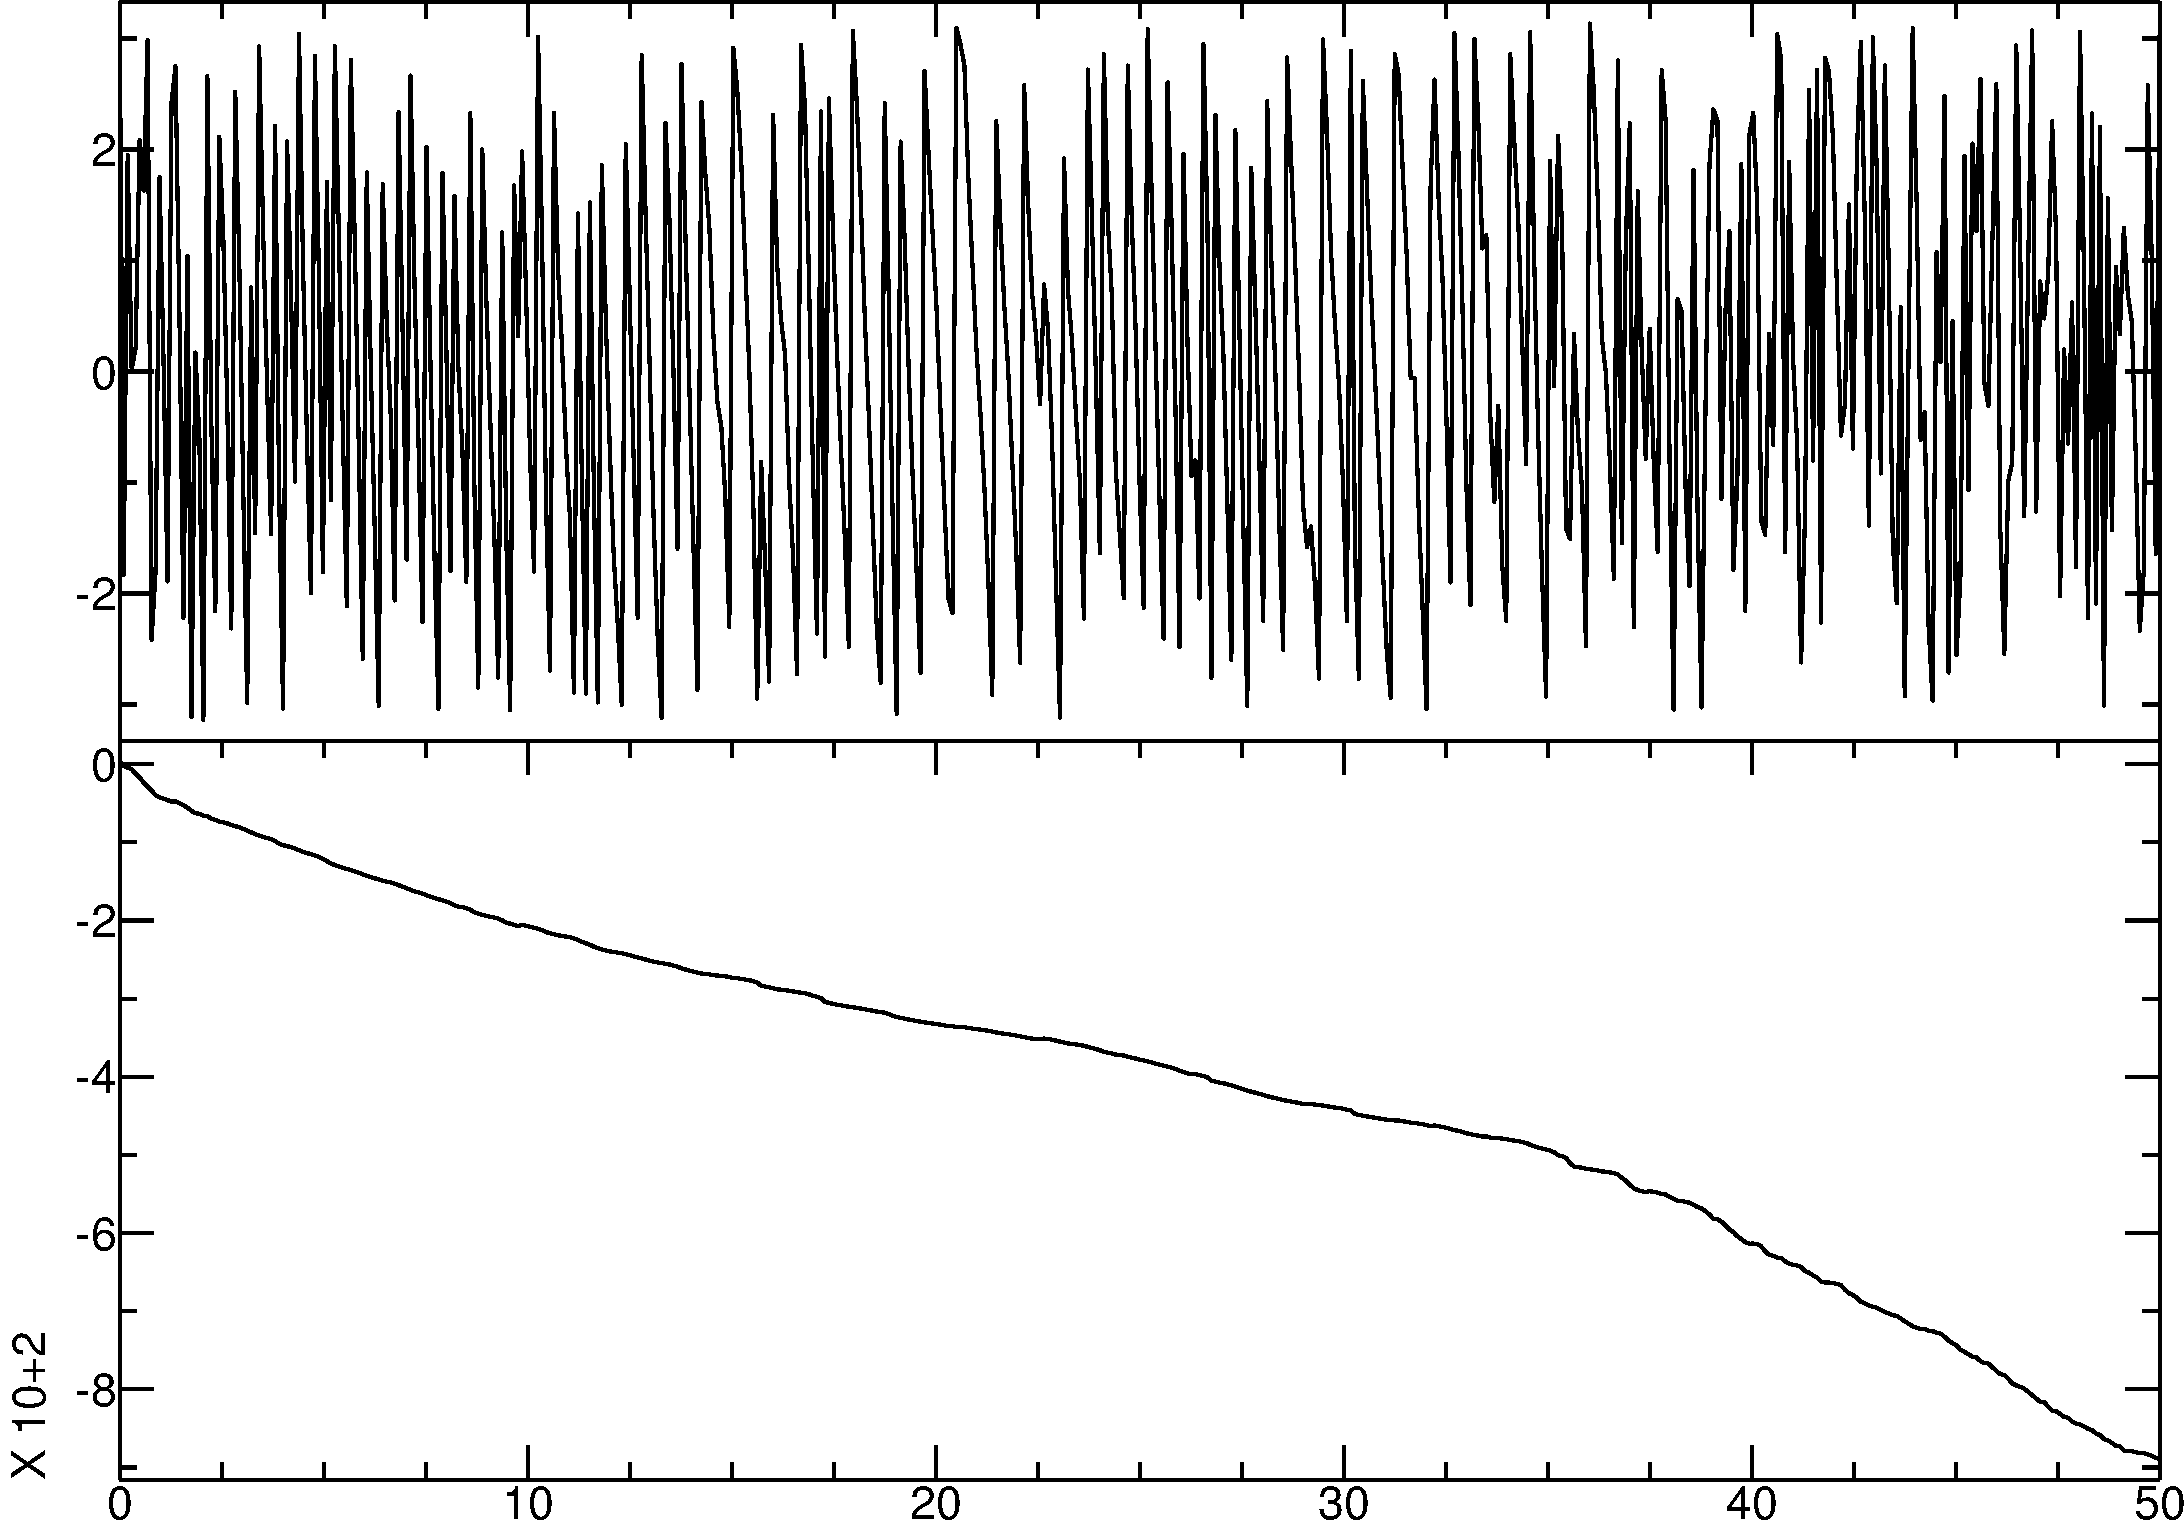
\includegraphics[width=0.9\textwidth]{unwrap}
\caption{展开相位}
\end{figure}

相位展开算法中使用了两种方法来估计每个频率处的展开相位。

一种是通过快速傅氏变换做相位偏导的数值积分。若要得到一个一致的估计,
则可将梯形积分的步长在每个频率上对分。可以使用 \texttt{INTTHR} 选项控制
这个验算的阈值,此值单位为弧度。减小 \texttt{INTTHR} 将改进相位计算结果,
若该值太小,会导致解的发散。

算法中使用的第二个方法是先用反正切函数计算相位的主值。展开相位的计算方法
是相位主值加上$2\pi$的整数倍,直到相位的突变小于给定的阀值为止。可以使用
\texttt{PVTHR} 选项控制这个验算的阀值。与上一个算法类似,减少这个阀值将
改进相位估算的结果,但也增加了无解的可能性。

这两个阀值的初值通常经验地取为:
\[ \pi/4 < PVTHR < INTTHR < 2\pi \]

\SACTitle{头段变量}
\texttt{b}、\texttt{e} 和 \texttt{delta} 分别改变为变换的起始频率、结束
频率和采样频率。原始的 \texttt{b}、\texttt{e} 和 \texttt{delta} 被保存
在为 \texttt{sb}、\texttt{se}、\texttt{sdelta},当进行反变换时将值带回。

\SACTitle{限制}
目前可以转换的数据最大长度为4096。
